
\section{The angle of Incidences influence on the headphone transfer function}

\subsection{Purpose}
The purpose of this experiment is to determine if the angle of incidence has any influence on the headphone transfer function and the cancellation path. 

The hypothesis is that the angle on incidence influences both the time delay and magnitude response of the transfer functions.

Measurements will only be performed in a horizontal plane. 

\subsection{AAU num list}
\begin{table}[H]
	\centering
	\ra{1.3}
	\begin{tabular}{ c c c } \toprule
		{Item}	& {Description} 						& {AAU-no}. \\ \bottomrule 
		1	&	B\&K Head And Torso Simulator "Henry" Type 4128	& 08453	\\
		2	&	B\&K ½'' Condenser Microphone Type 4134 	& XXXX		\\
		3	&	Beyerdynamic DT 770 Headphones				& XXXX		\\
		4	&	Soundcard RME Fireface 802					& 86838		\\
		5	&	Vision B3565 Computer running simulink		& NaN		\\
		6	&	B\&K Measuring Amplifier Type 2636			& 08717		\\
		7	&	B\&K Sound Calibrator Type 4230				& 08155		\\ 
		8	&	Small microphone							& XXXX		\\
		9	&	Genelec speaker								& TBD		\\ 
		10	&	Preamp for the small microphone	(homemade)	& TBD\\
		11	& 	B\&K Microphone Power Supply Type 2804		& 07304		\\
		\bottomrule
	\end{tabular}
	\caption{Table over equipment used in test.}
	\label{tab:AngleOfIncideceHP}
\end{table}

\subsection{Diagram}
\begin{figure}[H]
	\centering
	\begin{subfigure}[b]{.4\textwidth}
		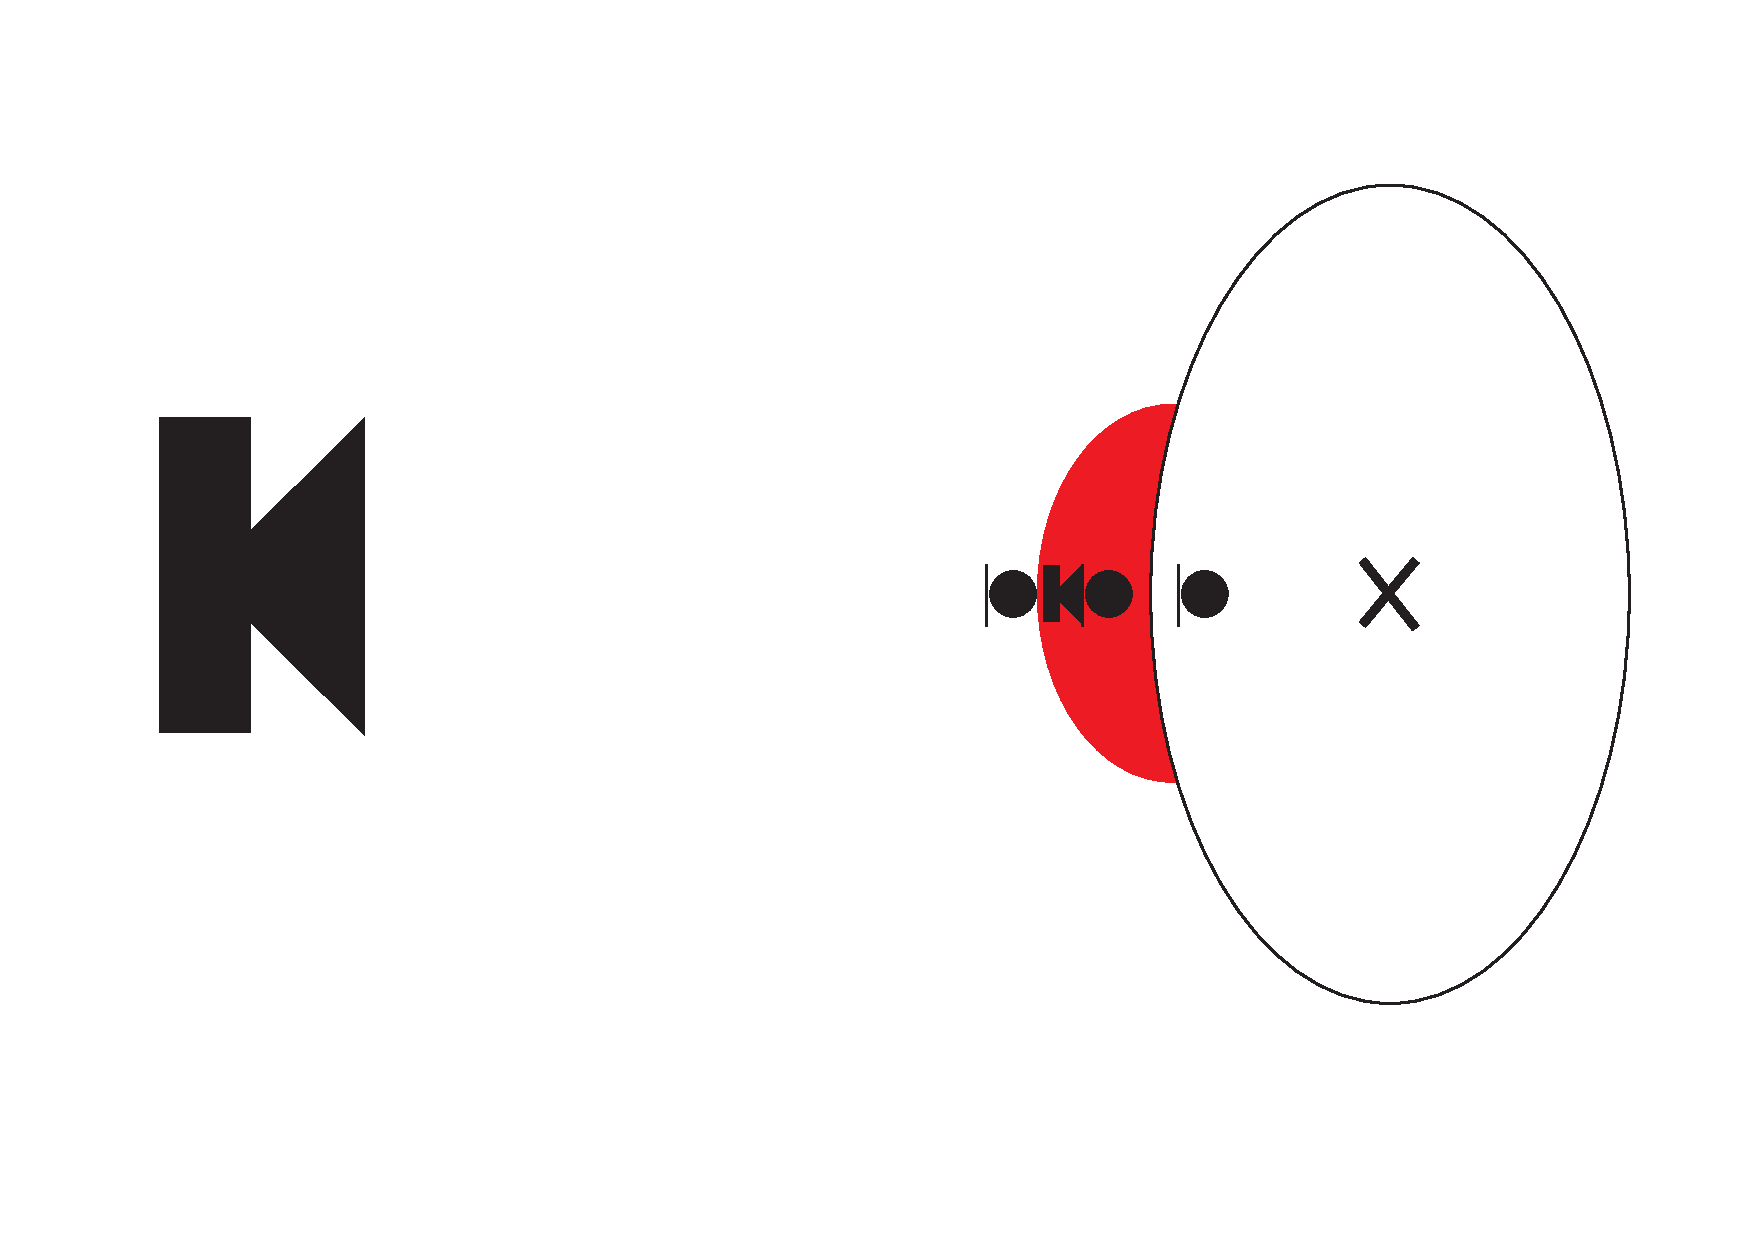
\includegraphics[width=\textwidth]{../Journal/Experiments/AngleOfIncidence/AngleOfIncidenceOnAxis.pdf}
		\caption{On axis}
		\label{fig:AngOfIndOnax}
		\vspace{2ex}
		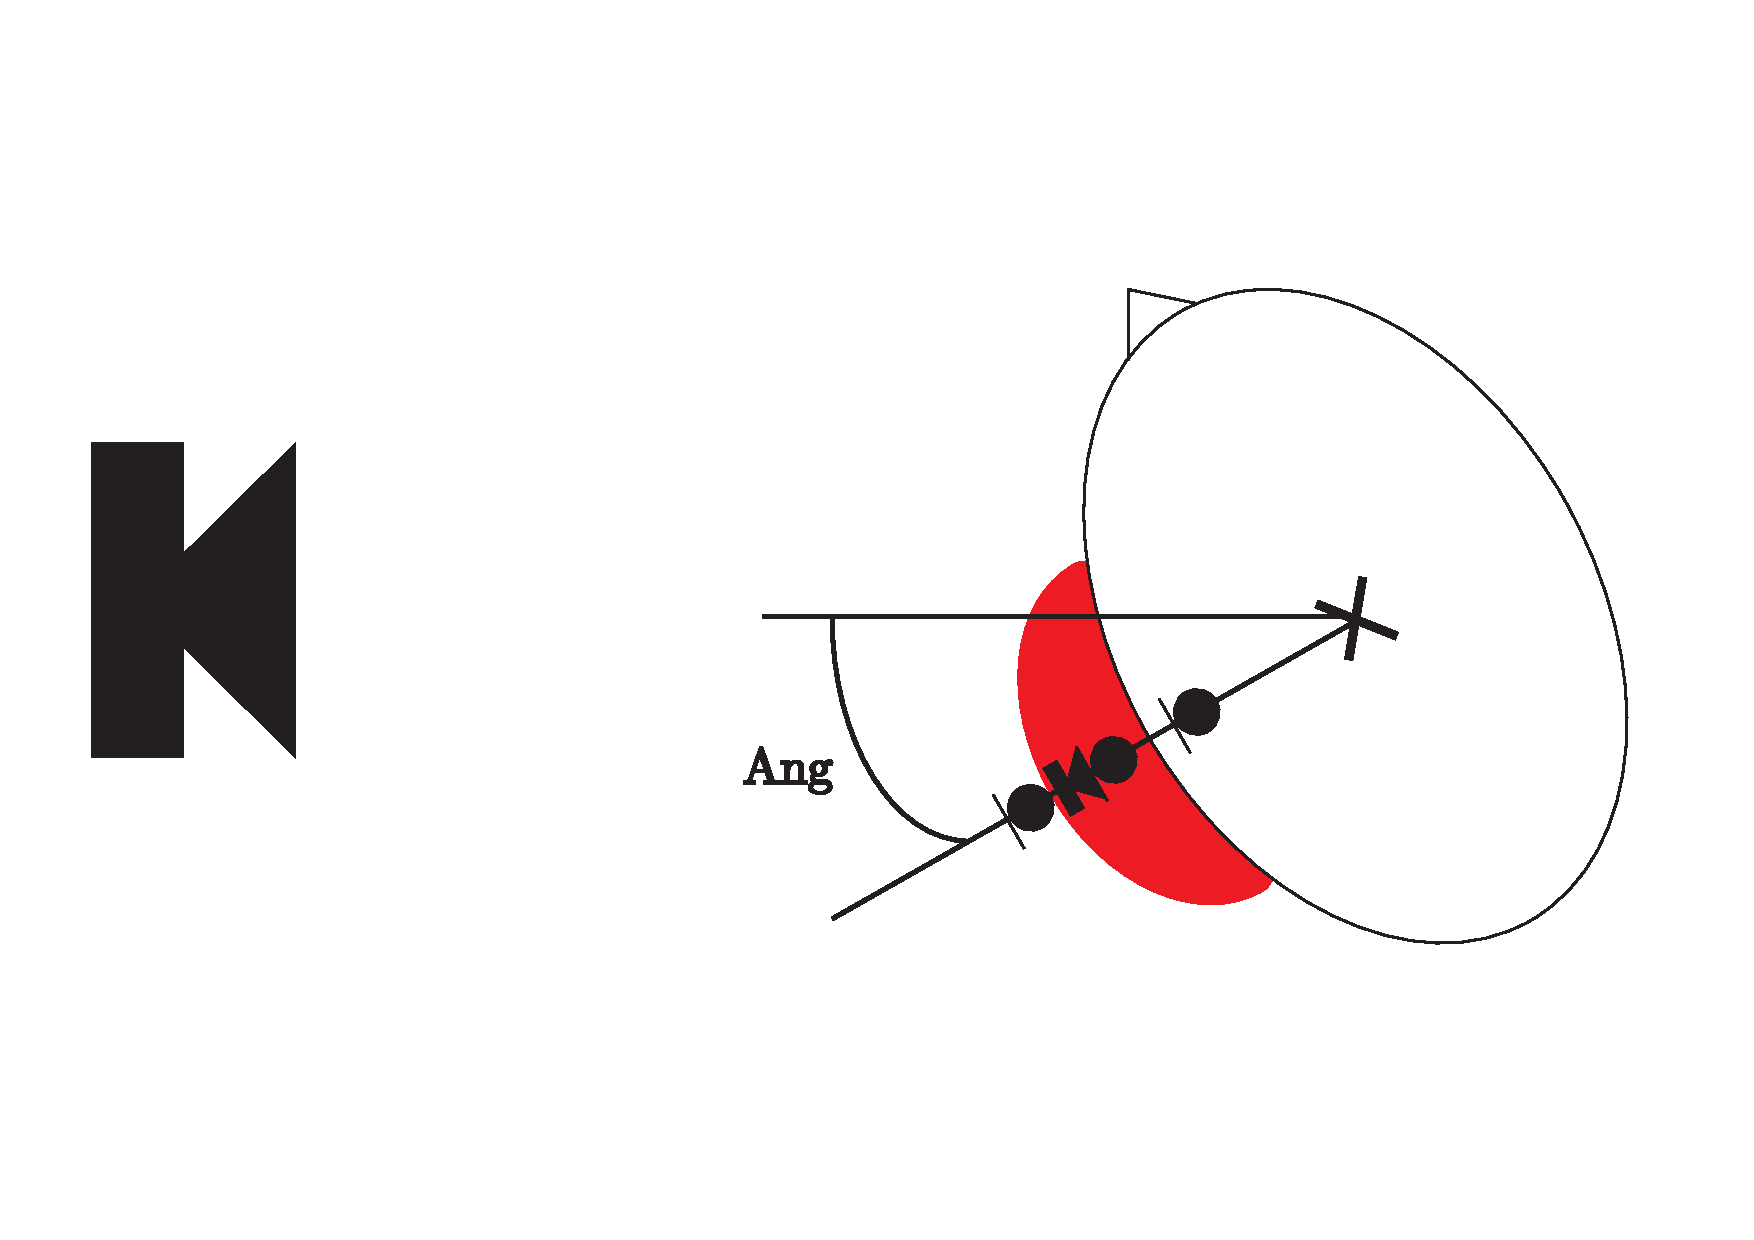
\includegraphics[width=\textwidth]{../Journal/Experiments/AngleOfIncidence/AngleOfIncidenceOffAxis.pdf}
		\caption{Off axis}
		\label{fig:AngOfIndOffax}
	\end{subfigure} 
	\begin{subfigure}[b]{.4\textwidth}
	\centering
	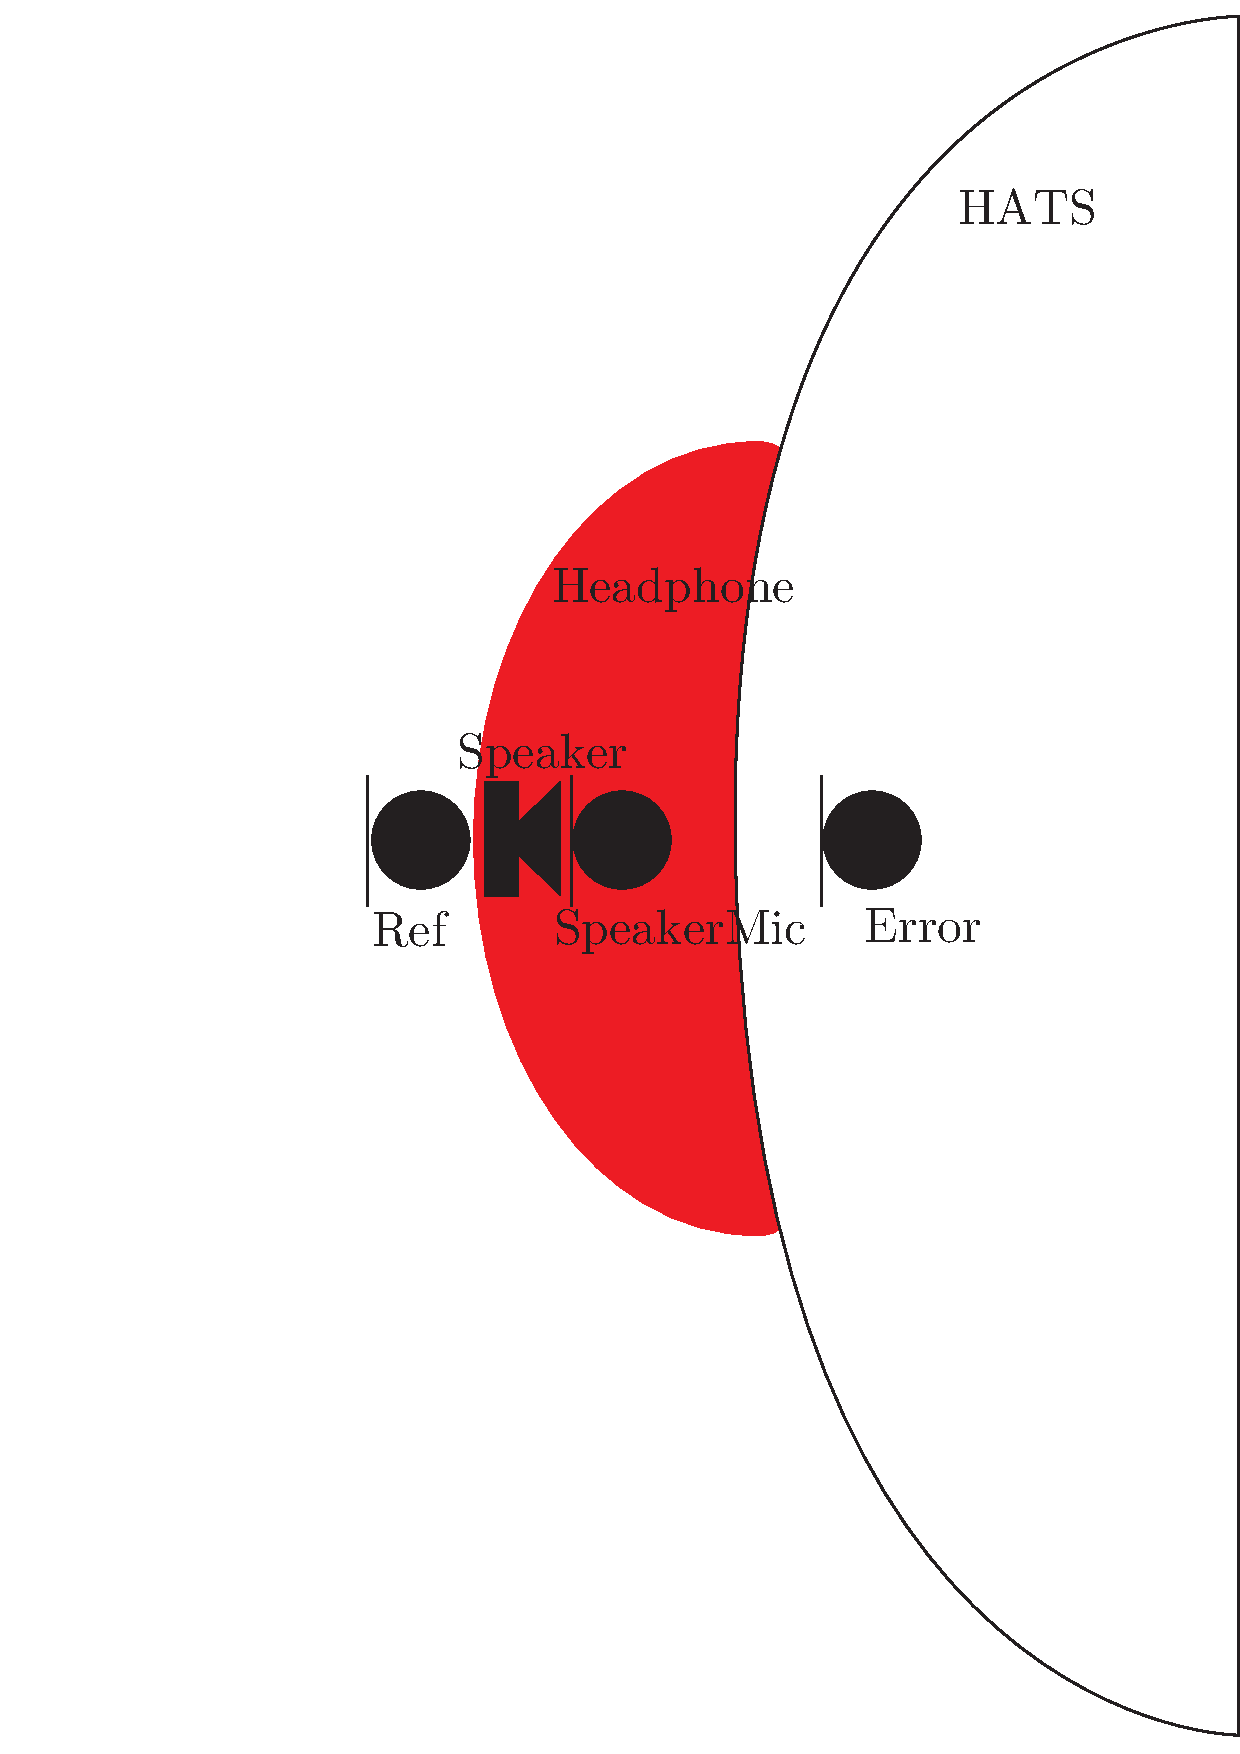
\includegraphics[width=\textwidth]{../Journal/Experiments/AngleOfIncidence/AngleOfIncidenceSchematic.pdf}
	\caption{Placement of microphones}
	\label{fig:AngOgIndMicplace}
\end{subfigure}
	\caption{Placement of microphones and rotation}
	\label{fig:AngleOfIndDiagram}
\end{figure}


\subsection{Settings/Description}
The experiment uses a single speaker to measure angles of incidence. Therefore either the speaker has to be moved around or the HATS will have to be turned to the right angles. \\
Adjusting the angle is done by rotating the HATS around the centre of the HATS leaving the speaker in place. This creates a triangle between the speaker, microphone and inner microphone of the HATS. The baseline of the triangle is from the microphone to the inner microphone, and angle is adjusted according to that line.
The following angles are examined:
\begin{table}[H]
	\centering
	\begin{tabular}{c c c c c c c c c c} \toprule
		0 & 10 & 20 & 30 & 40 & 50 & 60 & 70 & 80 & 90 \\ \bottomrule
	\end{tabular}
\label{Tab:AngleOfInciMeasAngles}
\caption{angles that measurements should be performed at. 0\textdegree is the situation in \autoref{fig:AngOfIndOnax}}
\end{table}
 
% The following Matlab code is used to calculate the angles at which measurements should be performed. The first measurement is performed at a 180\textdegree angle. This determines the length of the baseline (maxI in the code below). After determining the angles of interest can be calculated.  \\
%The script is based on two triangles that share a corner, the turning point, and a side to the speaker. The two triangles share the same angle at the turning point. This creates for two equations with two unknowns using the cosine relation and the fact that the side opposite the turning point should have a length "x" in one triangle and "x" + an amount of samples in the other triangle. Using this the angle can  be found.

\begin{figure}[H]
	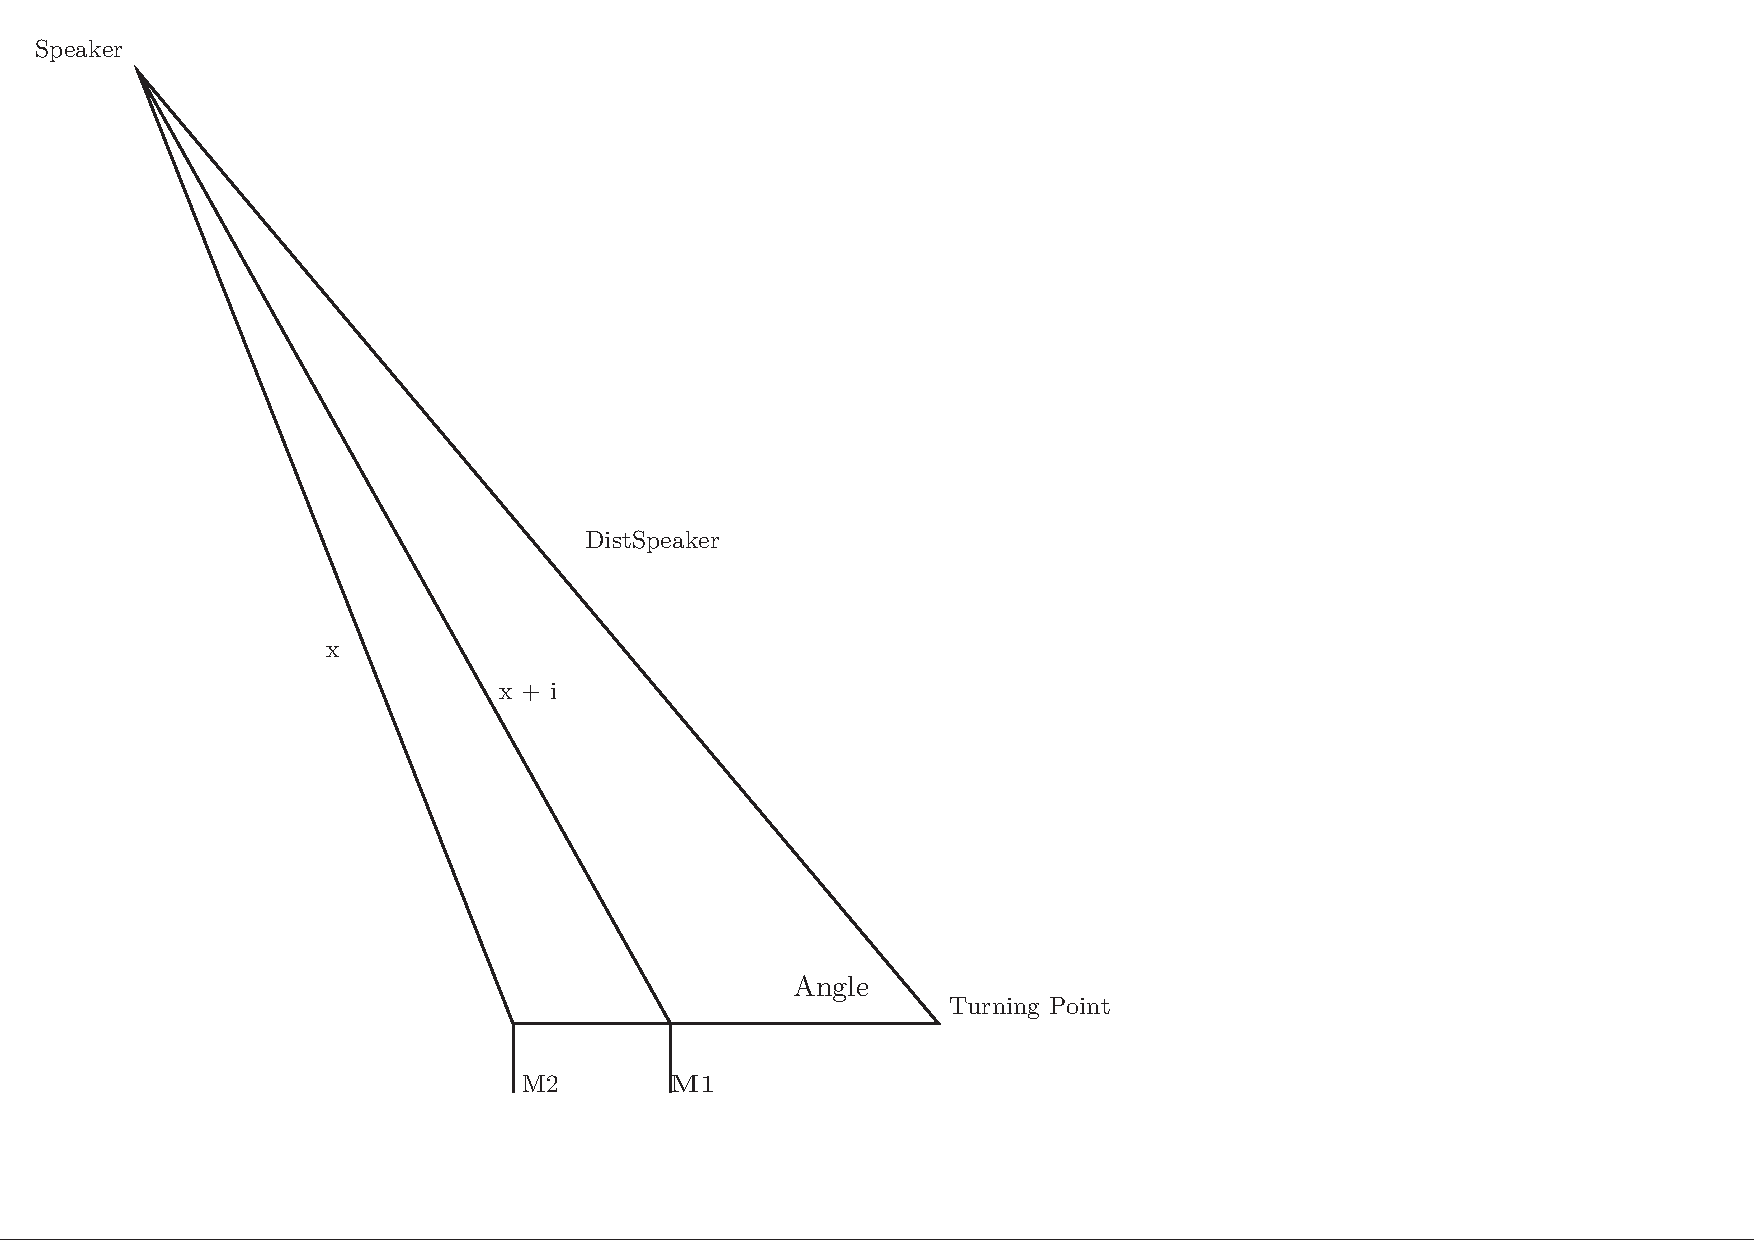
\includegraphics[width=\textwidth]{../Journal/Experiments/AngleOfIncidence/TriangleCalculation.pdf}
	\label{Fig:AngleOfIcidenceTriangleCalculation}
	\caption{The two triangle spanned by the centre og the Hats, the speaker and two of the microphones. M1 is the speakerMic and M2 is the Ref}
\end{figure}  


\subsection{Set-up}
\begin{figure}[H]
	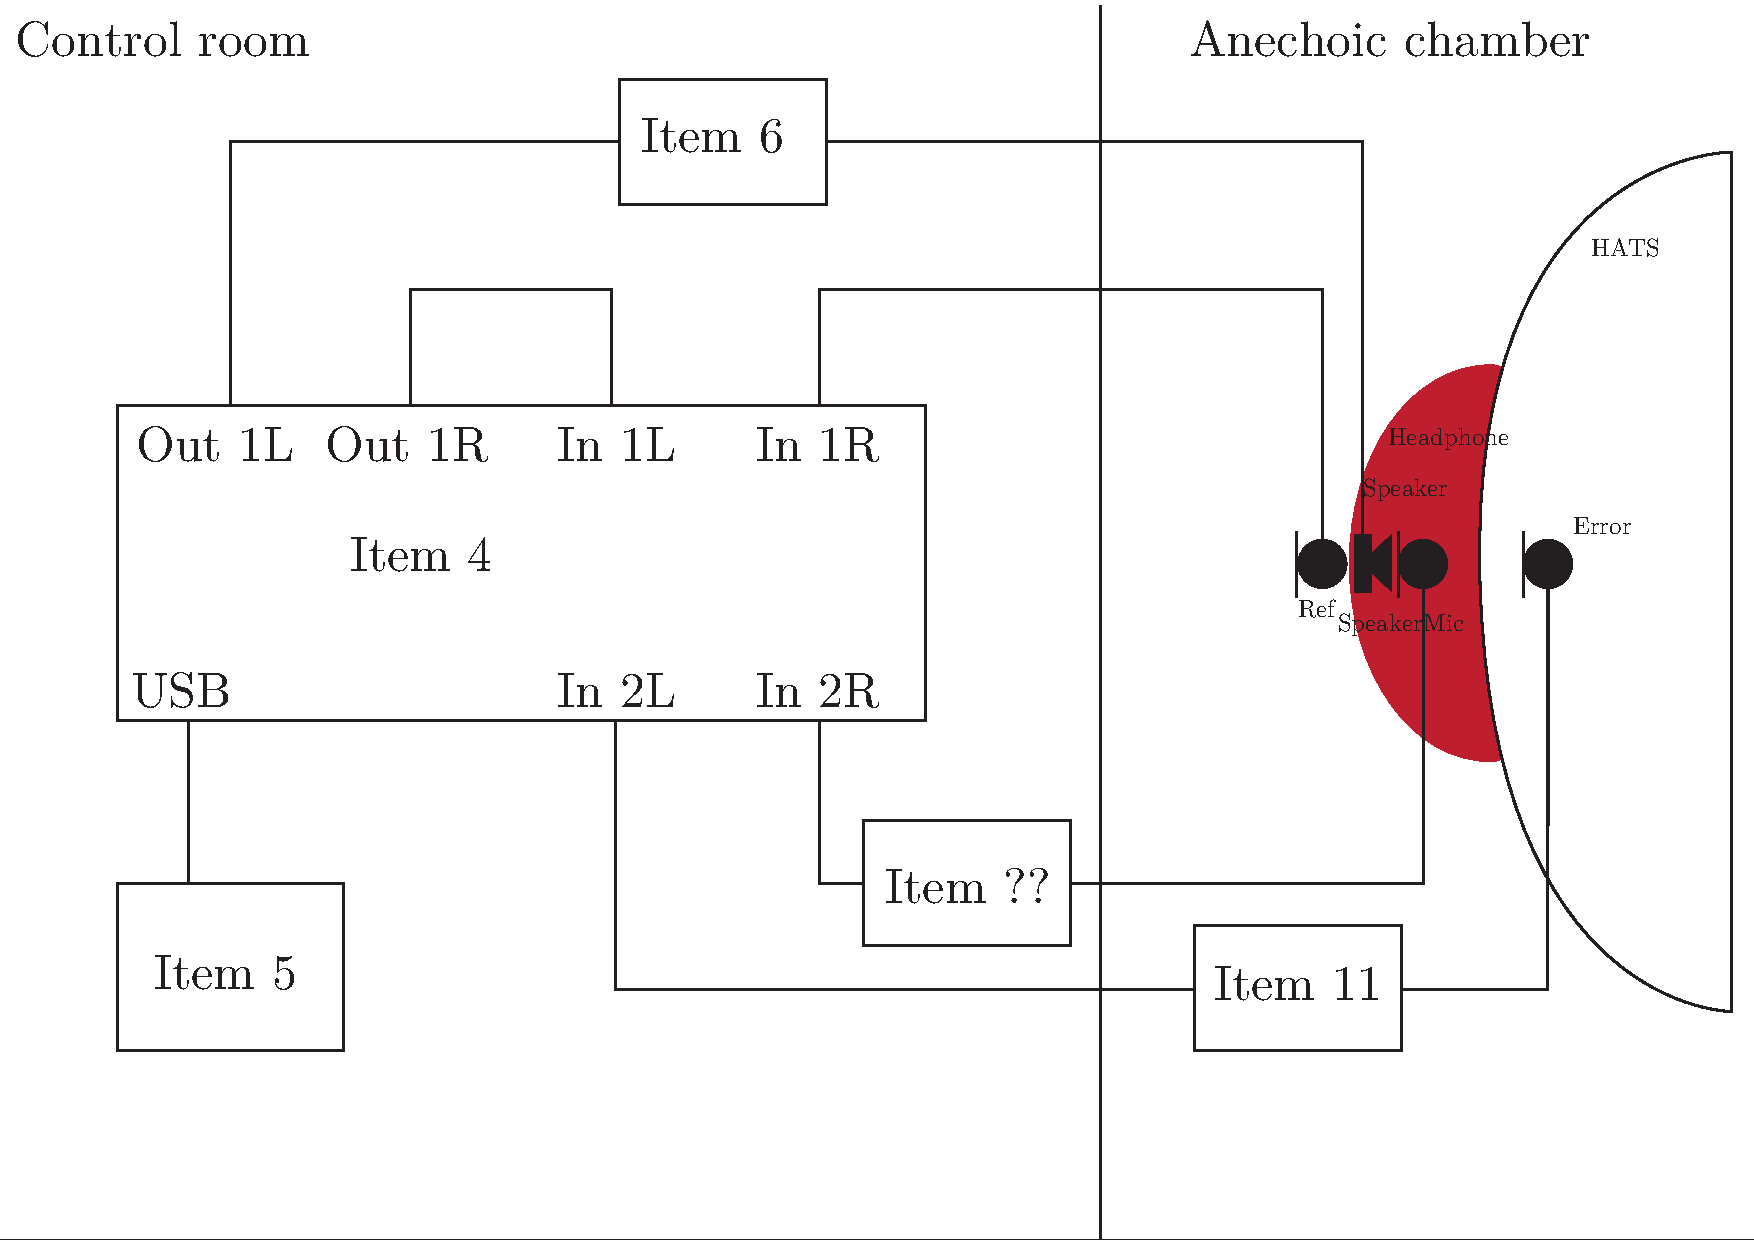
\includegraphics[width=\textwidth]{../Journal/Experiments/AngleOfIncidence/AngleOfIncidenceSetup.pdf}
	\caption{Setup of experiment on angle of incidence}
	\label{Fig:AngleOfIncidenceSetup}
\end{figure}

\subsection{Choice of equipment}
The experiment aims to be valid in the frequency range 20Hz to 20 kHz. This means that all equipment used should cover that frequency range. \\\\
The experiment uses a total of three microphones. The error microphone located inside the dummy's ear is given by the type fitted to the dummy. The SpeakerMic should be as small as possible in order to avoid influencing the transfer functions that are being measured. For this the very small XXXX is used. The Ref microphone has less restrictions on size and placement. This allows for the choice of a good standard measurement microphone, B\&K 4134. \\\\
For the speaker the limiting criteria is the lower roll off, especially in the anechoic chamber were reflections does not help a lot. However transfer functions between the microphones are measured, so absolute flatness is not critical. The Genelec XXXX is chosen. \\\\
The measurement system uses a RME Fireface 802 controlled using Simulink. Data extraction is made using the method described in \autoref{Sec:MeasATransFunc}

\subsection{Control and calibration}
The speaker is placed 1.6 meters from the centre of the HATS. \\\\
The two microphones SpeakerMic and Ref are fixed at distances 8.85 cm and 12.45 cm from the centre of the HATS respectively. The SpeakerMic is fitted just in front of the headphone speaker using medical tape.\\\\
For each microphone and pre-amplifier calibrations are made on the computer using Simulink\textsuperscript{\textregistered}.
\begin{itemize}
	\item For the Ref microphone calibration is made at 1000 Hz using the B\&K 4230 as calibrator. This should yield a signal of 93.6 dB as it is a pressure field microphone. The measured intensity in Matlab was XX so all measurements are multiplied by XXX to get a calibrated signal i Matlab. 
	\item For the Error microphone calibration is made at 1000 Hz using the B\&K 4230 as calibrator with adaptor B\&K 0741 for the ear of the HATS. This should yield a signal of 95.6 dB. The measured intensity in Matlab was XX so all measurements are multiplied by XXX to get a calibrated signal i Matlab. 
	\item For the speakerMic calibration is made using a earplug cut in half and fitted around the adaptor. This simple adaptor allows the B\&K 4230 to be used as calibrator. The measured output level is XXX, and should have been XXX. Therefore all measurements are multiplied by XXX to get a calibrated signal i Matlab. 
\end{itemize}
 
\subsection{Equipment settings}
\begin{itemize}
	\item This experiment is performed with a sampling rate of, $F_{s}$ = 48,000 Hz
	\item The Ref microphone is placed just outside the headset in-line with the ear and speaker unit. 
	\item The SpeakerMic is placed inside the headphone, as close to the speaker unit as possible. 
	\item For item 4 (sound card) take care to turn on the "inst" option in the mixing console. The following gain settings are present: 		
	\begin{itemize}
		\item Line level gain is 0 dB
		\item Error Microphones has gain XXXX
		\item Ref Microphones has gain XXXX
		\item Speaker Microphones has gain XXXX
	\end{itemize}
	\item Item 5 (computer) is set to 0 dBFS
	\item A logarithmic sine sweep is generated and saved in Matlab using the chirp function as follows:
	\begin{lstlisting} [language=Matlab	]
		IHope=10; % lala
	\end{lstlisting}
\end{itemize}

\subsection{Picture}
\begin{figure}[H]
	\includegraphics[width=\textwidth]{../Journal/Experiments/AngleOfIncidence/AngInSetup.jpg}
	\label{AngIncidenceSetup}	
	\caption{Setup of the experiment}
\end{figure}


\subsection{Procedure}
\begin{enumerate}
	\item Set the HATS at the angle under test. 
	\item Open Simulink\textsuperscript{\textregistered} and run file "SimulinkAngleOfIndence.xls"
	\item Run Simulink\textsuperscript{\textregistered} to play "LogChirp.wav" through the speaker
	\item Record and save, and name "Mic[i].wav", "SpM[i].wav", "loop[i].wav" and Ref[i].wav"\footnote{[i] indicates the angle of the experiment}
	\item Repeat the experiment for all angles.
\end{enumerate}

\subsection{Data Extraction}
The data is saved during the experiment

\subsection{Analysis}

\subsection{Error Sources}

\subsection{Conclusion}